\section{Generative models from differential equations}

We have said thousands of times before that our goal while training a ML algorithm is to minimize a loss function. However, we have never thought about this question in the previous sections: can we trust it? \textbf{Goodhart's law} states that "when a measure becomes a target, it ceases to be a good measure". This means that if we over-optimize an experiment or an algorithm to forcibly obtain a certain measure, we are probably going to get what we want, but that does not mean that such a measure has any significance. We should always remember that our loss function is just a proxy (a good one nonetheless) 
for model performance, not our ultimate goal. Here is a simple analogy:
\begin{itemize}
    \item[-] \textit{Objective}: Increase scientific knowledge.
    \item[-] \textit{Proxy}: Reward scientists for the number of papers.
    \item[-] \textit{Result}: Overproduction of papers and decline in quality of research.
\end{itemize}
Keep this in mind while approaching the next topic.

Notice also that all generative models that we encountered in the last sections have about the same basic structure shown below: starting from a latent space, a NN generates a distribution $\hat{p}(x)$ which is compared with the true data distribution $p(x)$ by the loss function during training.

\begin{center}
    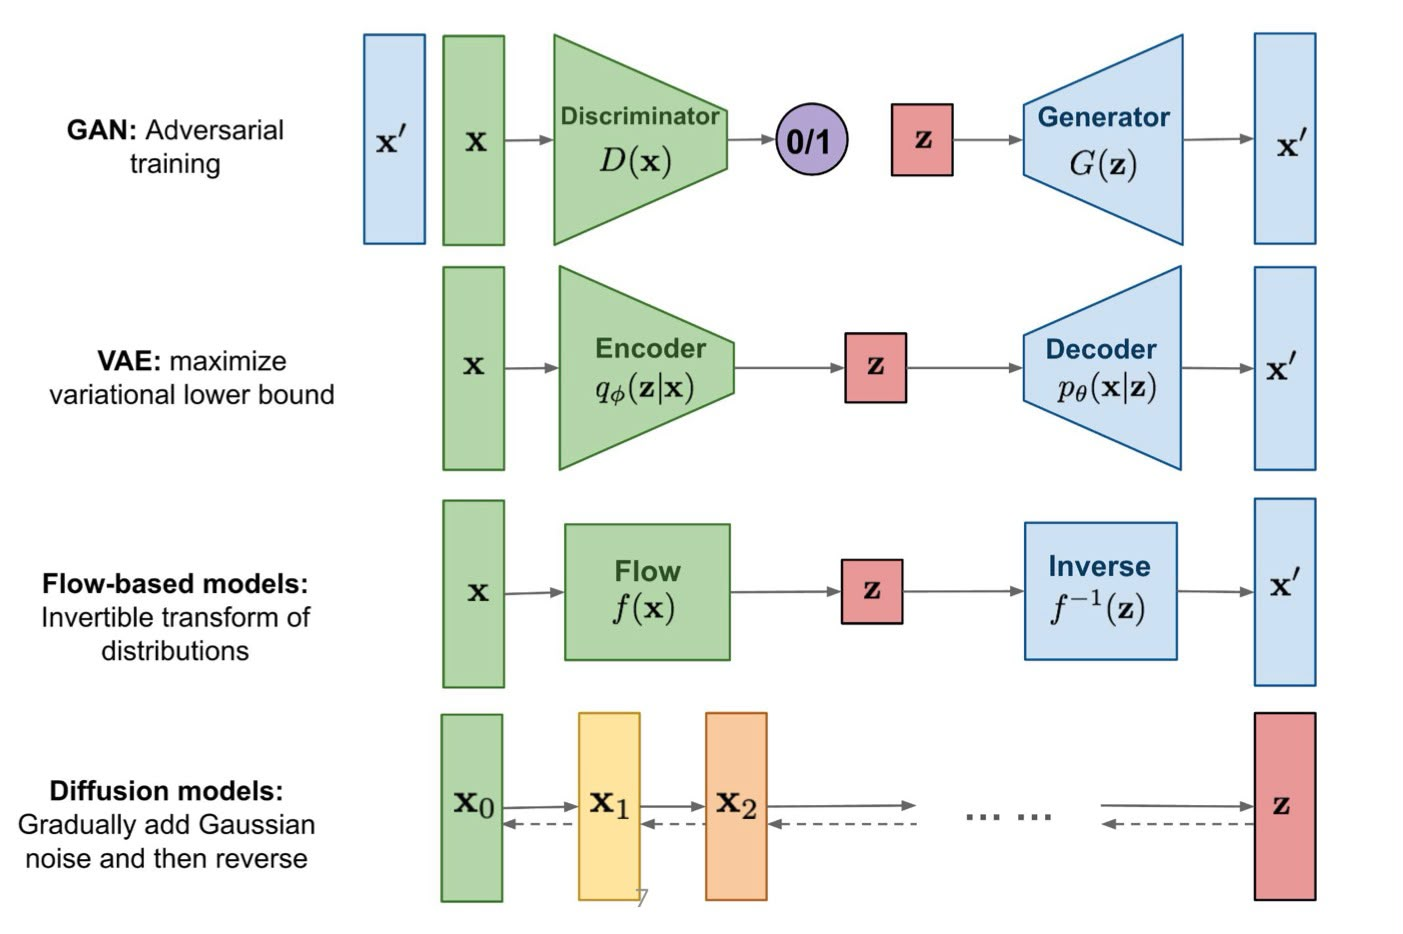
\includegraphics[width=0.49\textwidth]{figuresML_adv/lesson_ml_adv_3_pag_7.png}
    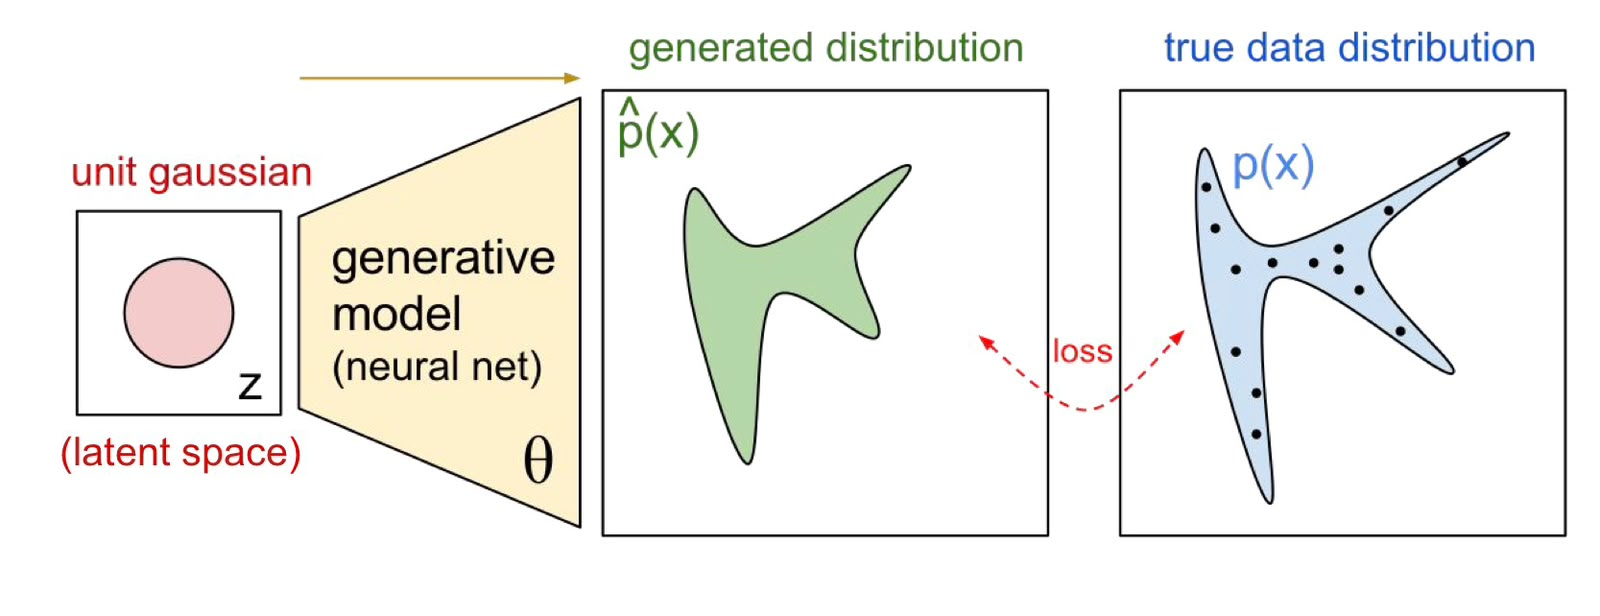
\includegraphics[width=0.49\textwidth]{figuresML_adv/lesson_ml_adv_3_pag_11.png}
\end{center}

Both research and industry are always craving faster, more flexible and expressive generative models and the results are still not perfect, especially in image/video generation (with models like Google Nano Banana and so on). A big improvement was made in 2023, as you can see by comparing these generated images of Will Smith eating spaghetti.

\begin{center}
    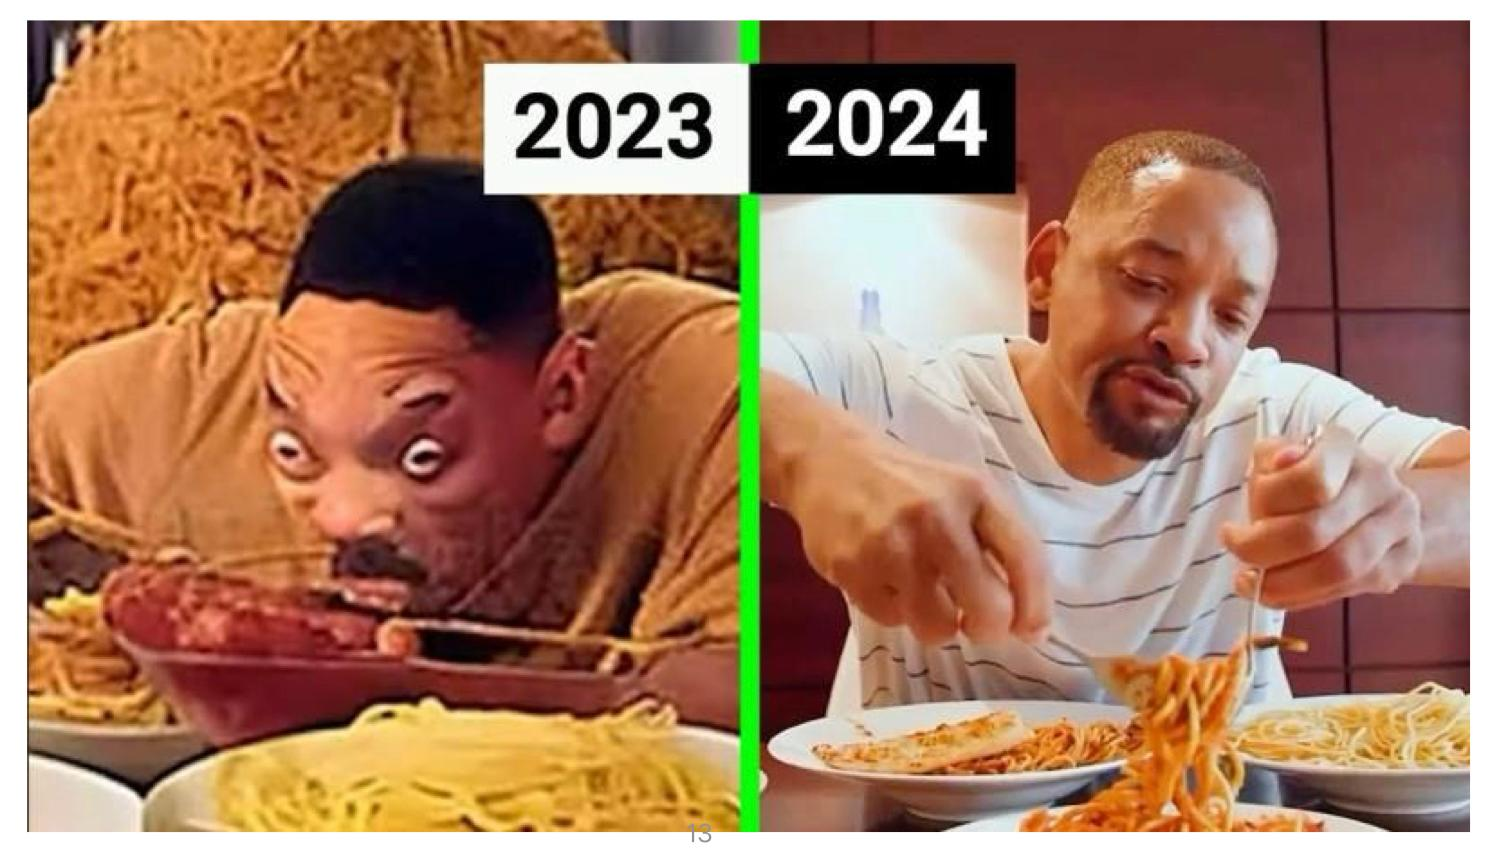
\includegraphics[width=0.55\textwidth]{figuresML_adv/lesson_ml_adv_3_pag_13.png}
\end{center}

What changed between 2023 and 2024? A new paradigm based on differential equations was implemented.

\subsection{From Ordinary Differential Equations to flow models}
Let $P_{init}$ be the distribution of our points in the latent space (e.g. $P_{init} \sim \mathcal{N}(0, I)$). The objective of a generative model is to send $P_{init}$ into a distribution $P_{data}$ in our data space depending on some parameters $\theta$ in our NN. To do so, people realized that Ordinary Differential Equations can be used. Let's go over some basics about them.

A time-dependent \textbf{vector field} is a continuous mapping $u: \mathbb{R}^d \times [0,1] \rightarrow \mathbb{R}^d$ that assigns a tangent vector (representing the instantaneous velocity) to every point $x \in \mathbb{R}^d$ at any given time $t \in [0,1]$. Given such a vector field, a \textbf{trajectory} (or integral curve) is a continuously differentiable curve $x: [0,1] \rightarrow \mathbb{R}^d, \ t \mapsto x_t$ such that its tangent vector at any time $t$ perfectly matches the vector field at that exact position and time. 

Therefore, an \textbf{Ordinary Differential Equation (ODE)}, and in particular its corresponding Cauchy problem, is written as:
\begin{equation}
    \begin{cases}
        \frac{dx_t}{dt} = u_t(x_t) \\
        x_0 = X_0 \quad \text{(initial condition)}
    \end{cases}
\end{equation}

We call \textbf{flow} (or flow map) the function $\psi: \mathbb{R}^d \times [0,1] \rightarrow \mathbb{R}^d$, $(x_0, t) \mapsto \psi_t(x_0)$. The flow describes the simultaneous evolution of the entire state space over time, parameterized by the initial conditions. It can be proven that if $u$ is continuously differentiable (or at least Lipschitz continuous, which guarantees the existence and uniqueness of the solution via the Picard-Lindelöf theorem, as typically assumed in ML algorithms), then $\psi$ is the unique solution of the ODE, satisfying:
\begin{equation}
    \begin{cases}
        \frac{\partial \psi_t(x_0)}{\partial t} = u_t(\psi_t(x_0)) \\
        \psi_0(x_0) = x_0
    \end{cases}
\end{equation}

These are all aspects of the same mathematical object: the vector field $u$ induces the ODE, the individual trajectories $x_t$ solve the ODE for specific starting points, while the flow $\psi$ is a continuous family of such solutions.

\begin{comment}
Let $x: [0,1] \rightarrow \mathbb{R}^d, \ t \rightarrow x_t$ be a trajectory in our data space $\mathbb{R}^d$ and $u: \mathbb{R}^d \times [0,1] \rightarrow \mathbb{R}^d$ a vector field that defines how to "move along" the trajectory. An ODE (in particular its corresponding Cauchy problem) is written as:
\begin{equation*}
    \begin{cases}
        \frac{dx_t}{dt} = u_t(x_t) \\
        x_0 = x_{0} \quad \text{(initial condition)}
    \end{cases}
\end{equation*}

We call \textbf{flow} the function $\psi: \mathbb{R}^d \times [0,1] \rightarrow \mathbb{R}^d$, $(x_0, t) \rightarrow \psi_t(x_0)$ and it can be proven that if $u$ is \textbf{continuously} differentiable % as it should in ML algorithms
then $\psi$ is a solution of the ODE:
\begin{equation*}
    \frac{\partial \psi_t}{\partial t}(x_0) = u_t(\psi_t(x_0))
\end{equation*}
These are all aspects of the same mathematical object: $u$ induces the ODE, the trajectories $x_t$ solve the ODE, while a flow is a family of solutions.
\end{comment}

Now, what does this have to do with ML? Since our goal is to move from a point sampled from $P_{init}$ to one sampled from $P_{data}$, we can identify the first with the initial condition $x_0$ of an ODE, and the latter with a point $x_1$ of the same trajectory. We can then arrive at the definition of a so-called \textbf{flow model}, which is a neural network $u_t^\theta$ that satisfies:
\begin{equation}
    \begin{cases}
        \frac{dx_t}{dt} = u_t^\theta(x_t) \\
        x_0 = X_0
    \end{cases}
\end{equation}
where $\theta$ are the trainable parameters.

\begin{center}
    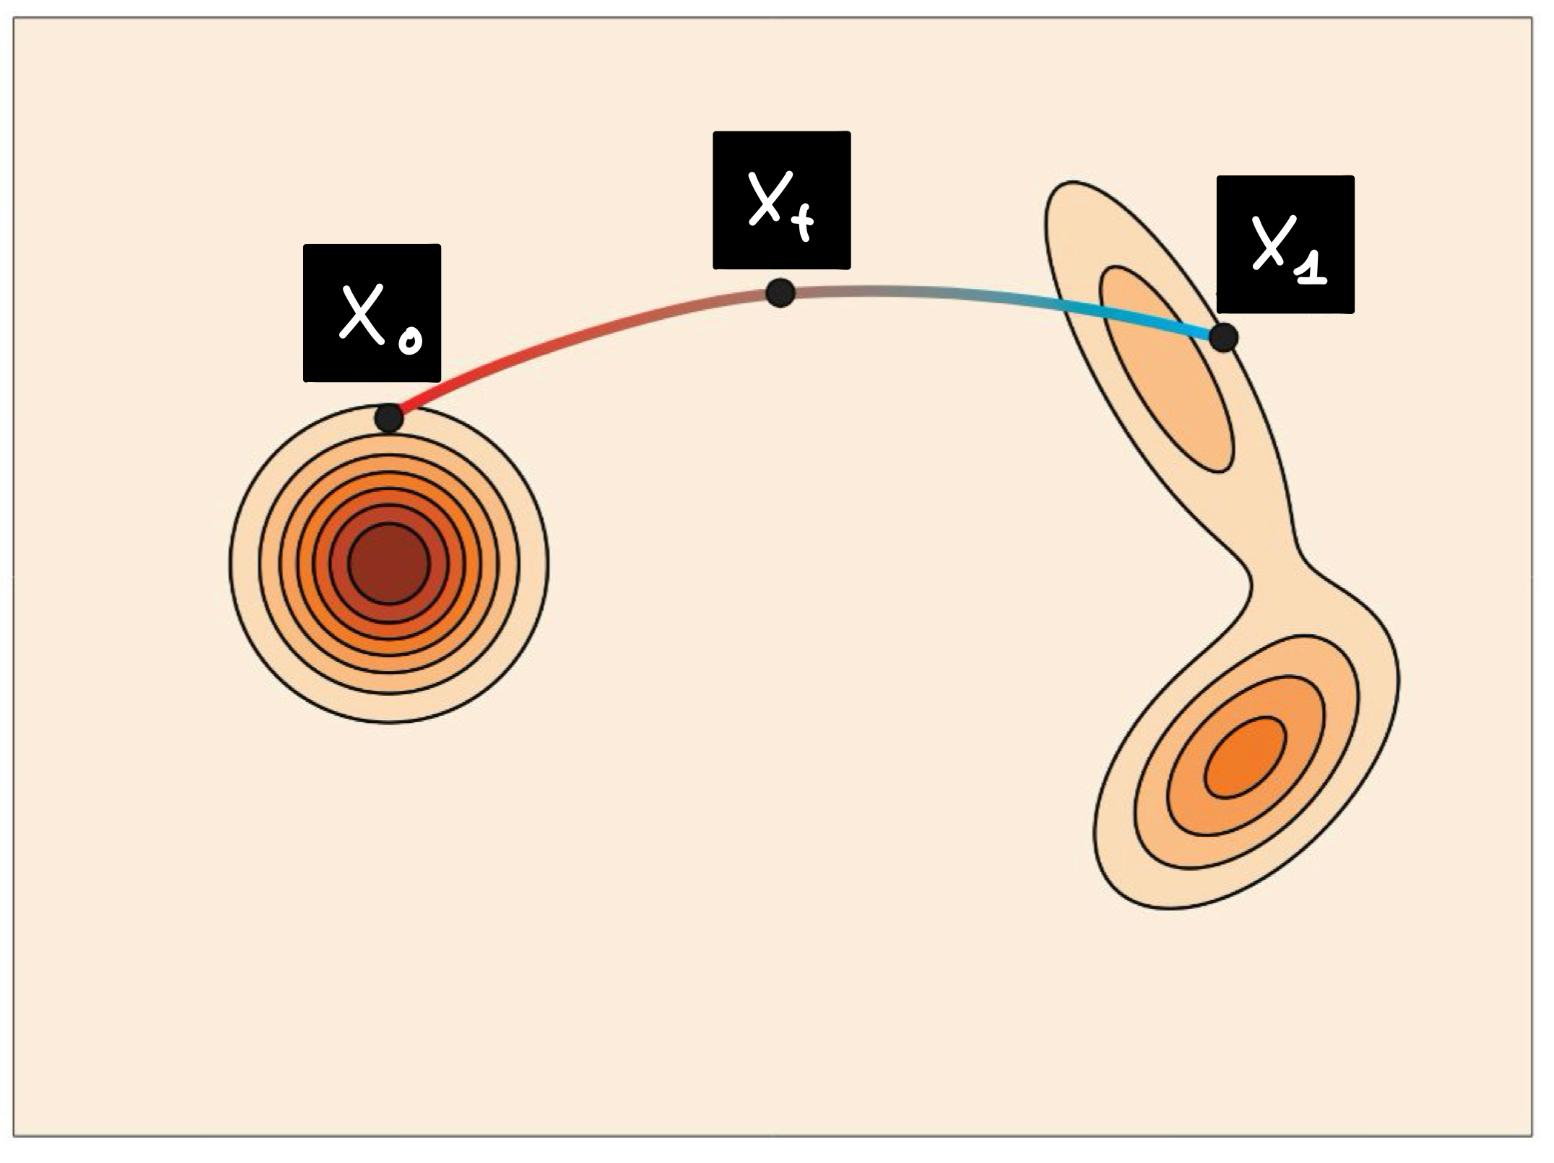
\includegraphics[width=0.45\textwidth]{figuresML_adv/lesson_ml_adv_3_pag_16.png}
\end{center}

Pay attention: even if it is called "flow model", $u_t^\theta$ is actually a vector field  with parameters $\theta$ (by our previous definitions) which takes a data point and the corresponding time and returns a velocity ($\mathbb{R}^d \times [0,1] \rightarrow \mathbb{R}^d$). 

Our main question now becomes clear: how can I create a NN such that the flow that passes through the initial point $\psi_1^\theta(x_0)$ is sampled from $P_{data}$ if computed at $t=1$?

It is fundamental to notice that in this case, \textit{the term "latent space" is just a semantic relic from older models}: in reality the two distributions live in the exact same space and with latent space we can refer to the cloud of starting points. 

For example, if we are working with images $256 \times 256 \times 3$, then our data space would be $\mathbb{R}^{196608}$, just as our latent space. Only a small part of such space is known, i.e. the points corresponding to our training dataset. Given those, we want to train our NN to move from a cloud of normally distributed points ($P_{init} \sim \mathcal{N}(\mu, \sigma)$, which in practice are just images full of random noise, like an old TV with no signal) to the ones corresponding to the images we want to generate ($P_{data}$). 
This movement (schematically represented in the figure below) means solving the "right" ODE defined by the "right" vector field, i.e. our NN.

\begin{center}
    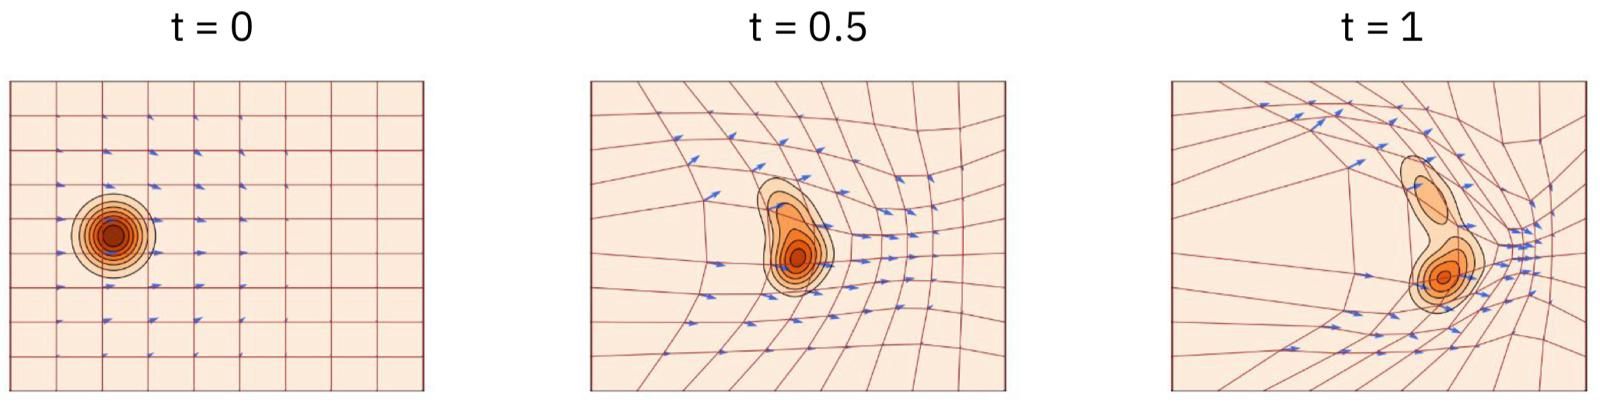
\includegraphics[width=0.8\textwidth]{figuresML_adv/lesson_ml_adv_3_pag_18.png}
\end{center}

\hrulefill

\textbf{Note: From Ordinary Differential Equations to flow models}

While ODEs are used to define flow models, another powerful class of equations called \textbf{Stochastic Differential Equations (SDEs)} forms the mathematical backbone of another ML paradigm: \textbf{diffusion models}. The general form of an It\^o SDE is given by:
\begin{equation}
    dx_t = u_t(x_t) \, dt + \sigma_t \, dW_t
\end{equation}
where $u_t(x_t)$ is called the \textit{drift coefficient} (a deterministic vector field governing the macroscopic movement of the data) and $\sigma_t > 0$ is the \textit{diffusion coefficient}. The term $dW_t$ represents the infinitesimal increment of a standard \textit{Wiener process} (or \textit{Brownian motion}), which continuously injects stochastic noise into the system, effectively causing the state to undergo a random walk. 

Rigorously, a $d$-dimensional standard Wiener process $W_t$ is a continuous-time stochastic process characterized by the following properties:
\begin{enumerate}
    \item $W_0 = 0$ almost surely;
    \item $W_t - W_s \sim \mathcal{N}(0, (t-s)I)$ for $0 \leq s < t$;
    \item The random variable $(W_{t_2} - W_{t_1})$ is independent from $(W_{t_4} - W_{t_3})$ for $0 \leq t_1 < t_2 \leq t_3 < t_4$.
\end{enumerate}
The second condition specifies that the increments of the process are normally distributed with zero mean and a variance that scales linearly with the time step $(t-s)$. The third condition ensures that the increments over non-overlapping intervals are strictly independent.

Because of the injected noise, the solution to an SDE is not a deterministic curve but a \textit{stochastic process}, more precisely a diffusion process or a random-walk. Consequently, every time we solve the equation from the same starting point, the corresponding realization (or sample path) will yield a different, inherently noisy trajectory, as shown in the figure.

\begin{comment}
If ODEs are used to define flow models, there is another class of equations called \textbf{Stochastic Differential Equations (SDEs)} that get us to yet another ML paradigm: \textbf{diffusion models}. The general form of a SDE is the following:
\begin{equation*}
    dx_t = u_t(x_t)dt + \sigma_t dW_t
\end{equation*}
where $\sigma_t > 0$ is called diffusion coefficient while $dW_t$ is the rate of change of a Brownian noise, which essentially injects noise in our solutions causing a random walk. In particular, $W_t$ is an object such that:
\begin{equation*}
    \begin{cases}
        W_0 = 0 \\
        (W_t - W_s) \sim \mathcal{N}(0, (t-s)I) \\
        (W_t - W_s) \ \text{is independent from every other} \ (W_v - W_u) 
    \end{cases}
\end{equation*}
The second condition means that differences between $W$ values at different times of the same process, are distributed as a gaussian distribution with variance that increases with the time interval.

The solution of a SDE is a stochastic process and the corresponding trajectories will change at every iteration as shown in figure.
\end{comment}

\begin{center}
    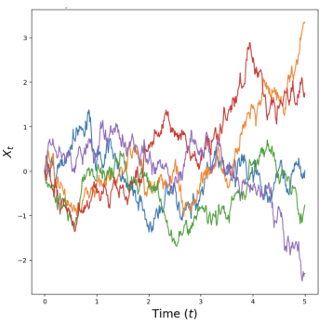
\includegraphics[width=0.3\textwidth]{figuresML_adv/lesson_ml_adv_3_brown.png}
\end{center}

A diffusion model will then be defined by a vector field $u_t^\theta(x_t)$ (the NN) such that
\begin{equation}
    dx_t = u_t^\theta(x_t) \, dt + \sigma_t \, dW_t
\end{equation}
and a diffusion coefficient usually set at a constant value $\sigma_t = \sigma > 0$.

Given the randomness of diffusion models, with such algorithms it is easier to explore the space of solutions. However, experts are slowly realizing that flow models can be just as expressive as their stochastic counterparts.

\hrulefill

\subsection{The long road to flow matching}
Ideally, what we are trying to achieve is just a regression to a target solution $\tilde{u}_t(x_t)$ which would like to be analytically computable from the ODE. This means that our loss function could simply be written as the MSE:
\begin{equation*}
    \mathcal{L}(\theta) = ||u_t^\theta(x_t) - \tilde{u}_t(x_t)||^2
\end{equation*}
Of course, if we knew $\tilde{u}_t(x_t)$ analytically there would be no need to search for $u_t^\theta(x_t)$, so this is certainly not the right reasoning.

In order to find a suitable training target, we need to introduce another object called \textbf{conditional probability path}. Let $y \in \mathbb{R}^d$ be a point in the data space (sampled from $P_{data}$). The conditional probability path of the variable $x \in \mathbb{R}^d$ given $y$ as a function of time ($t \in [0,1]$) is a set $\{P_t(x|y)\}_{t \in [0,1]}$ of probability distributions such that:
\begin{equation*}
    \begin{cases}
        P_0(x|y) = P_{init}(x) \\
        P_1(x|y) = \delta(x-y)
    \end{cases}
\end{equation*}
In other words, as time increases, the distributions of the path "shrink" around the value of $y$, as shown in figure.

\begin{center}
    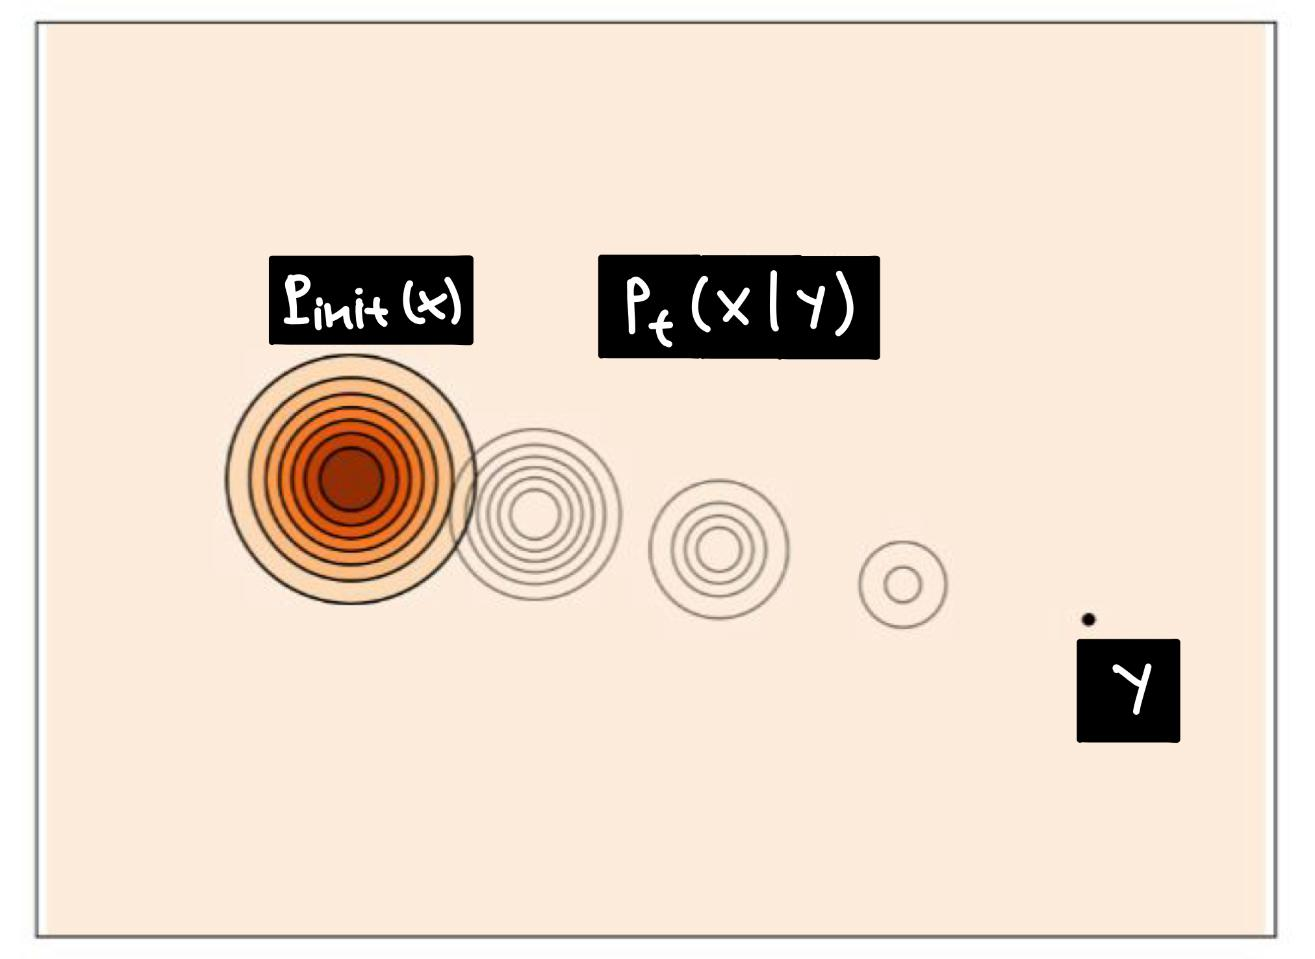
\includegraphics[width=0.45\textwidth]{figuresML_adv/lesson_ml_adv_3_pag_24.png}
\end{center}

A fundamental example is the \textbf{Gaussian conditional probability path}:
\begin{equation}
    P_t(x|y) = \mathcal{N}(\alpha_t y, \beta_t^2 I_d)
\end{equation}
with $\alpha_t, \beta_t$ scalar functions of time. % chosen by us for example
Imposing the 2 conditions above we get:
\begin{equation*}
    \begin{cases}
        P_0(x|y) = \mathcal{N}(\alpha_0 y, \beta_0^2 I_d) = P_{init}(x) = \mathcal{N}(0, I_d) \\
        P_1(x|y) = \mathcal{N}(\alpha_1 y, \beta_1^2 I_d) = \delta(x-y)
    \end{cases}
\end{equation*}
These equations are true if we take $\alpha_t = t$ and $\beta_t = 1-t$, which gives
\begin{equation}
    P_t(x|y) = \mathcal{N}(ty, (1-t)^2 I_d)
\end{equation}
If we then sample $x$ from this probability path we get points distributed in this way:
\begin{equation}
    x_t = \alpha_t y + \beta_t \epsilon = ty + (1-t)\epsilon
\end{equation}
where $\epsilon$ is just random Gaussian noise ($\epsilon \sim \mathcal{N}(0, I_d)$). Of course $x_t \rightarrow y$ for $t \rightarrow 1$, as it should.

Now, notice again what any conditional probability path does: it sends points sampled from the distribution $P_{init}$ into a single point $y$, or similarly $P_{init}$ into $\delta(x-y)$. That is not exactly what we wanted, right? We want the initial points in the latent space to transform into the corresponding generated data points (or analogously $P_{init}$ to "become" $P_{data}$ at $t=1$). 

That can be achieved thanks to the so-called \textbf{marginal probability path} defined as the set $\{P_t(x)\}_{t \in [0,1]}$ such that:
\begin{equation}
    P_t(x) = \int \, dy \ P_t(x|y) P_{data}(y)
\end{equation}
This is an integral over all the possible values of $y$, in other words an \textit{average} over all the possible outcomes of the transformation starting from $x$. That is exactly what we needed, as the marginal probability path is what "moves" $P_{init}$ to $P_{data}$. To better understand this, take a look at what happens at $t=0$ and $t=1$:
\begin{itemize}
    \item[-] At $t=0$: \\ $P_0(x) = \int \,dy \ P_0(x|y) P_{data}(y) = P_{init}(x) \int P_{data}(y) \, dy = P_{init}(x)$
    \item[-] At $t=1$: \\ $P_1(x) = \int \,dy \ P_1(x|y) P_{data}(y) = \int \,dy \ \delta(x-y) P_{data}(y) = P_{data}(x)$
\end{itemize}

That is the perfect tool for our purposes, and the two examples in these next figures should make it even more clear. However, there is an obvious problem: $P_t(x)$ depends on $P_{data}(y)$, which is what we are trying to find, so we cannot actually compute it. 

\begin{center}
    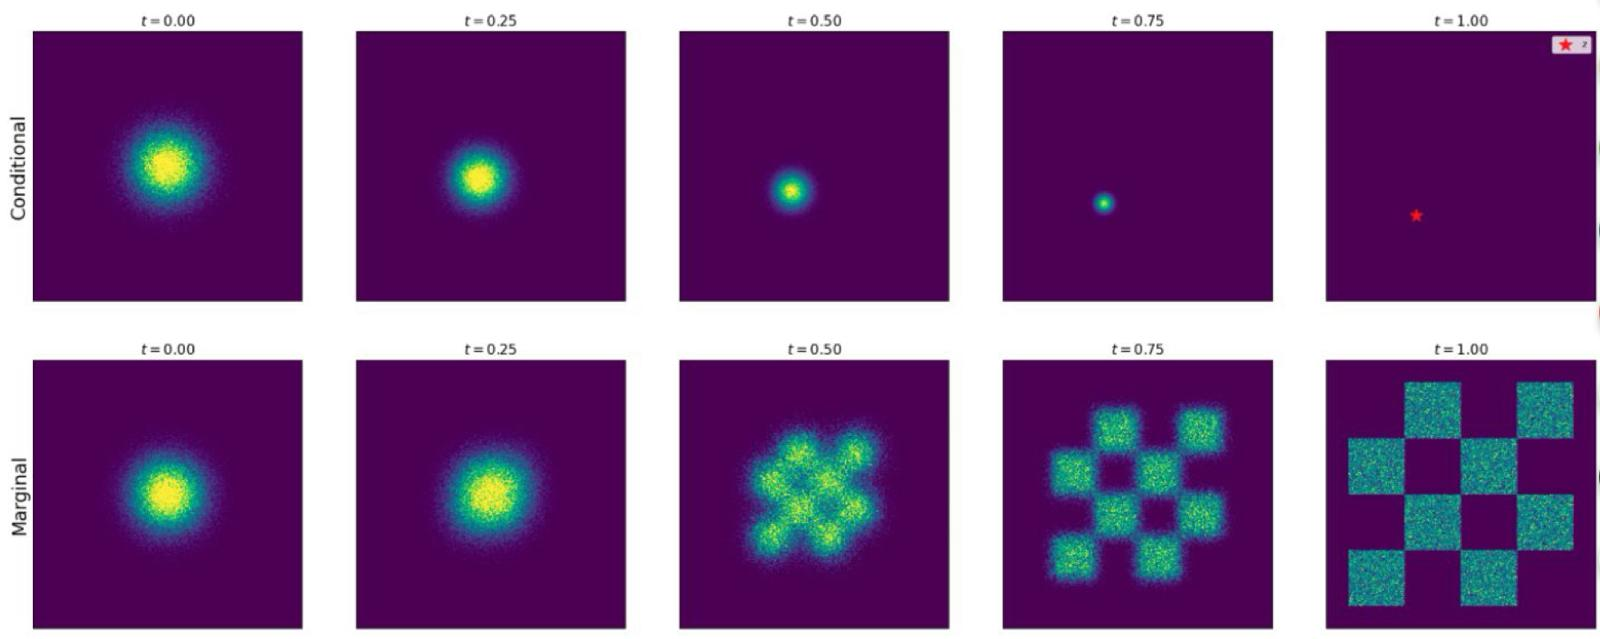
\includegraphics[width=0.9\textwidth]{figuresML_adv/lesson_ml_adv_3_pag_27.png}
    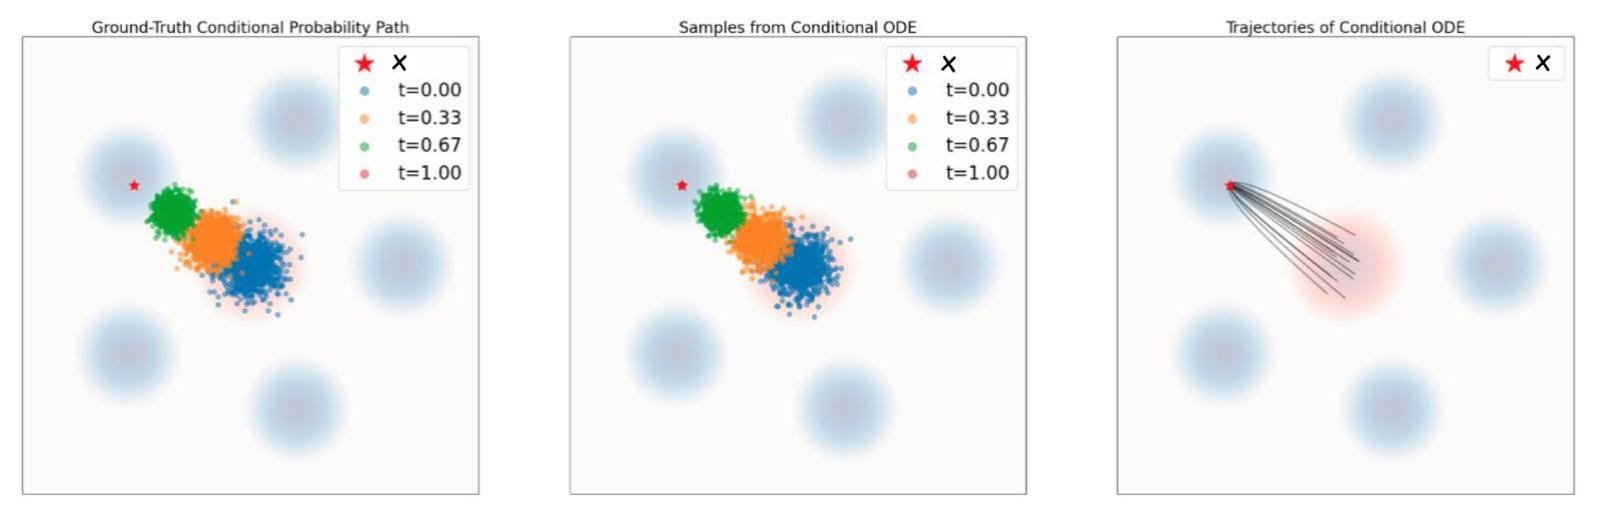
\includegraphics[width=0.9\textwidth]{figuresML_adv/lesson_ml_adv_3_pag_28.png}
\end{center} 

From what we have said up to now, understanding the meaning of these next definitions should come naturally. \\
A \textbf{conditional vector field} is a vector field $u_t^{target}(x|y)$ such that the corresponding ODE follows the conditional probability function, i.e.
\begin{equation}
    \frac{dx_t}{dt} = u_t^{target}(x_t|y) \quad \Rightarrow \quad  x_t \sim P_t(x|y)
\end{equation}
namely if $x_t$ is a solution of the ODE, then it is sampled from $P_t(x|y)$.

Just like before, a pivotal example is that of a \textbf{Gaussian conditional vector field}, which has the following form (you can easily find the explicit computation in the literature):
\begin{equation}
    u_t^{target}(x|y) = \left(\dot{\alpha}_t - \frac{\dot{\beta}_t}{\beta_t}\alpha_t\right)y + \frac{\dot{\beta}_t}{\beta_t}\epsilon
\end{equation}
and with $\alpha_t = t$ and $\beta_t = 1-t$:
\begin{equation}
    u_t^{target}(x|y) = y - \epsilon \quad \text{with } \epsilon \sim \mathcal{N}(0, I_d)
\end{equation}
This means that if we are moving along the conditional probability path from the initial distribution to the data point, the vector field that imposes this transformation is simply the difference between the point sampled from the noise and the data point itself, or, in other words, that we are following a straight path (see figure). In literature these paths are also called \textbf{optimal transfer paths}.

\begin{center}
    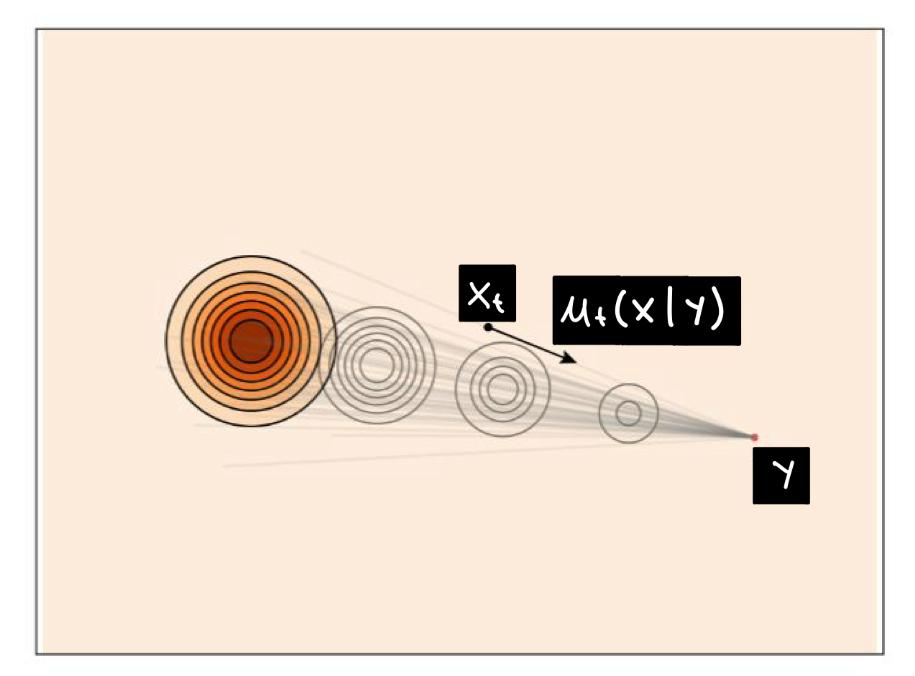
\includegraphics[width=0.45\textwidth]{figuresML_adv/lesson_ml_adv_3_pag_25.png}
\end{center}

Following the same logic as before (we want $P_{init}$ to go in $P_{data}$ not in a single point etc\dots) we analogously define the \textbf{marginal vector field} $u_t^{target}(x)$:
\begin{equation}
\begin{aligned}
    u_t^{target}(x) &= \int \,dy \ u_t^{target}(x|y) \frac{P_t(x|y) P_{data}(y)}{P_t(x)} \\
    &= \int \,dy \ u_t^{target}(x|y) P_t(y|x)
\end{aligned}
\end{equation}
where we applied Bayes' Theorem to obtain the second line.
\begin{center}
    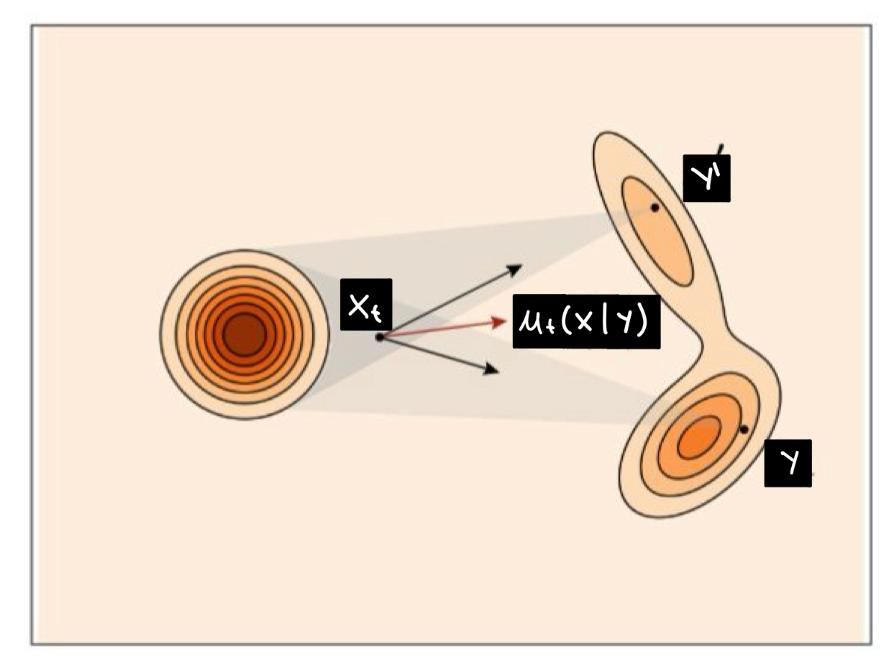
\includegraphics[width=0.45\textwidth]{figuresML_adv/lesson_ml_adv_3_pag_26.png}
\end{center}

From this comes a fundamental theorem usually referred to as the \textbf{marginalization trick}: if the conditional vector field $u_t^{target}(x|y)$ induces an ODE from which follows the conditional probability path $P_t(x|y)$, then the marginal vector field $u_t^{target}(x)$ defined by the integral induces in the same way the marginal probability path $P_t(x)$:
\begin{equation*}
    u_t^{target}(x|y) \rightarrow P_t(x|y) \quad \Rightarrow \quad u_t^{target}(x) \rightarrow P_t(x)
\end{equation*}

Again, we are getting closer and closer to a solution, but $u_t^{target}(x)$ still depends on the unknown $P_{data}$ so we are still facing an unsolvable problem in the purely analytical sense. We could attack it numerically, but then our training would become extremely slow, since we would need to solve the $u^{target}(x)$ integral for each training data point. This will all be very useful, but we still need another piece of the puzzle.

Fortunately, one more theorem comes to our aid. Let $x_0$ be our initial point sampled from $P_{init}$ and consider the ODE 
\begin{equation*}
    dx_t = u_t^\theta(x_t) \,dt   
\end{equation*}
where $u_t^\theta$ is our NN and $x_t$ is such that $x_1$ is sampled from $P_{data}$. Let's also define the \textbf{flow matching loss function} $\mathcal{L}_{FM}(\theta)$:
\begin{equation}
    \mathcal{L}_{FM}(\theta) = \mathbb{E}_{t \sim U[0,1], \ x \sim P_t(x)} \left[ ||u_t^\theta(x) - u_t^{target}(x)||^2 \right] \quad \text{\% expected value}
\end{equation}
where $\mathbb{E}$ is the expected value operator. \\
Just like before, if we knew $u^{target}(x)$ there would be no need for $u_t^\theta(x)$. So $\mathcal{L}_{FM}(\theta)$ cannot actually be computed. We can however compute the \textbf{conditional flow matching loss} $\mathcal{L}_{CFM}(\theta)$, defined as:
\begin{equation}
    \mathcal{L}_{CFM}(\theta) = \mathbb{E}_{t \sim U[0,1], \ y \sim P_{data}, \ x \sim P_t(x|y)} \left[ ||u_t^\theta(x) - u_t^{target}(x|y)||^2 \right]
\end{equation}
Even if it is computable, this seems apparently useless for our purposes. However, the following theorem solves all of our doubts: $\mathcal{L}_{CFM}(\theta)$ and $\mathcal{L}_{FM}(\theta)$ are exactly equal up to a \textbf{constant} $C \in \mathbb{R}$ which does not depend on the parameters $\theta$, i.e.
\begin{equation}
    \mathcal{L}_{CFM}(\theta) = \mathcal{L}_{FM}(\theta) + C \quad \text{, } C \in \mathbb{R}
\end{equation}
This means that:
\begin{equation}
    \nabla_\theta \mathcal{L}_{CFM}(\theta) = \nabla_\theta \mathcal{L}_{FM}(\theta)
\end{equation}
so minimizing $\mathcal{L}_{CFM}(\theta)$ automatically minimizes $\mathcal{L}_{FM}(\theta)$, which is what we need.

{ \small
\underline{Proof:} \\
We can expand the squares inside the modules:
\begin{align*}
    \mathcal{L}_{FM}(\theta) &= \mathbb{E} \left[ ||u_t^\theta(x)||^2 - 2u_t^\theta(x)^T u_t^{target}(x) + ||u_t^{target}(x)||^2 \right] \\
    \mathcal{L}_{CFM}(\theta) &= \mathbb{E} \left[ ||u_t^\theta(x)||^2 - 2u_t^\theta(x)^T u_t^{target}(x|y) + ||u_t^{target}(x|y)||^2 \right]
\end{align*}
We have to show that $$\mathbb{E}[u_t^\theta(x)^T u_t^{target}(x)] = \mathbb{E}[u_t^\theta(x)^T u_t^{target}(x|y)]$$ in order to prove that $$\nabla_\theta \mathcal{L}_{FM}(\theta) = \nabla_\theta \mathcal{L}_{CFM}(\theta)$$ In fact, those are the only two terms inside the expected value operator that are different and depend on $\theta$. By definition of expected value we have:
\begin{align*}
    \mathbb{E}[u_t^\theta(x)^T u_t^{target}(x)] &= \int_0^1 \,dt \int \,dx \ P_t(x) u_t^\theta(x)^T u_t^{target}(x) \\
    &= \int_0^1 \,dt \int \,dx \ P_t(x) u_t^\theta(x)^T \left[ \int \,dy \ u_t^{target}(x|y) \frac{P_t(x|y) P_{data}(y)}{P_t(x)} \right] \\
    &= \int_0^1 \,dt \int \,dx \int \,dy \ u_t^\theta(x)^T u_t^{target}(x|y) P_t(x|y) P_{data}(y) \\
    &= \mathbb{E}_{t \sim U[0,1], \ y \sim P_{data}, \ x \sim P_t(x|y)} [u_t^\theta(x)^T u_t^{target}(x|y)]
\end{align*}
which is exactly what we wanted to show. }

Let's get to our final result then, which is the selection of our perfect training target: we can train our network by minimizing a conditional flow matching loss that has the optimal transfer paths $u_t^{target}(x|y) = y - \epsilon$ as its training target:
\begin{equation}
    \mathcal{L}_{CFM}^{OT}(\theta) = \mathbb{E} \left[ ||u_t^\theta(x) - (y - \epsilon)||^2 \right] \quad \text{with } \epsilon \sim \mathcal{N}(0, I_d)
\end{equation}
As you can see, this is an extremely easy loss to write, implement and minimize. In this way the NN learns the ODE transforming the noise to data, as represented below.

\begin{center}
    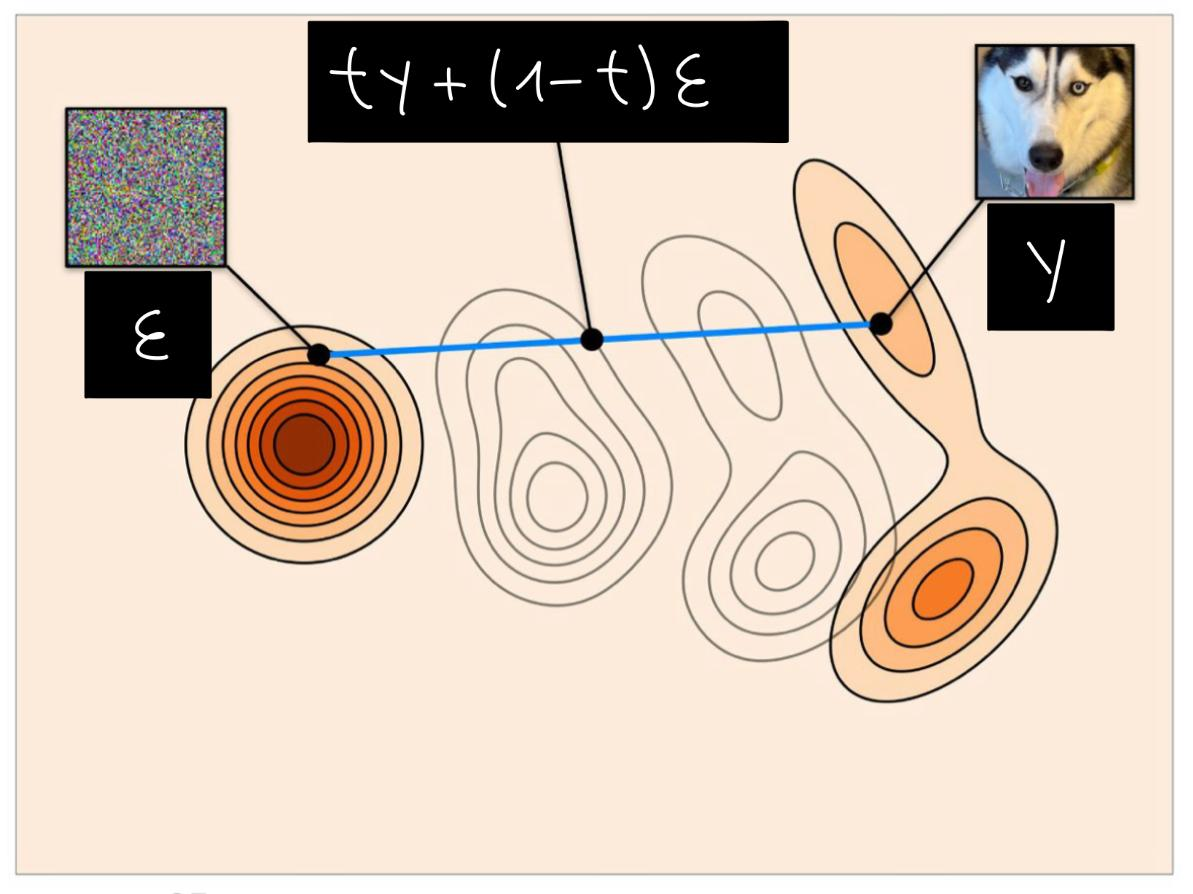
\includegraphics[width=0.45\textwidth]{figuresML_adv/lesson_ml_adv_3_pag_35.png}
\end{center}

\subsection{Applications of flow matching}
Industrial applications of these new ML paradigms revolve around image and video generation. As a flexible, expressive and powerful form of generative model, these algorithms are suitable for a broad range of tasks, for example:
\begin{itemize}
    \item[-] \underline{Fast simulation of detectors.} The greatest example of this application is what happens at the LHC, where flow models are used to run simulations of particle collisions to prove or disprove some theories. Roughly speaking, LHC will show a read-out that corresponds to the aftermath of a collision, but to reconstruct what caused that readout, you are going to need to create models based on different theories. With the advent of flow models, slow and costly numerical simulations are being substituted by ML algorithms, with a speed-up of 2-3 orders of magnitude.
    \item[-] \underline{Anomaly detection.} Flow models model the PDF of points based on ODEs, which are invertible. In other words, this means that given a new data point $y$, you can reconstruct back the corresponding $x$ in the latent space. If the point deviates from the expected initial distribution (i.e. has a low likelihood) it can be marked as an anomaly. This too is used in LHC to select the events of interest between the $4 \cdot 10^{16}$ collisions per second through trigger systems, which reduce this number to about $\sim 10^5$ events per second.
    \item[-] Many more applications to every task where you need to move from one probability space to another (super resolution, image reconstruction, and thousands of others).
\end{itemize}

As for every generative NN that models the probability density function, the generation can be made conditional (just like it is done with models like ChatGPT and so on).

For a deeper introduction to flow models look at \url{https://diffusion.csail.mit.edu/2025/index.html}.